% ----------------------------------------------------------
% Aplicação
% ----------------------------------------------------------
\chapter{Aplicação}
\label{chap:aplicacao}

De modo a avaliar o sistema de \textit{software} desenvolvido com base na metodologia apresentada, 
foi desenvolvido um modelo simplificado \textbf{baseado} em um sistema físico existente, no caso,
o reator TRIGA IPR-R1 do CDTN. A elaboração deste modelo levou em consideração os aspectos físicos
de um único elemento combustível - envolvido por certa quantidade de água - do reator TRIGA
em condições de utilização usuais de trabalho.

\section{Reator TRIGA IPR-R1}
\label{sec:triga}

%Nesta seção, será brevemente descrito o reator TRIGA IPR-R1, utilizado como referência para a
%construção do modelo simplificado utilizado na avaliação do sistema acoplado implementado nesta
%tese.

Os reatores do tipo TRIGA\textregistered (\textit{Training, Research and Isotopes}),
desenvolvidos pela \textit{General Atomics} (GA), são os mais utilizados
reatores de pesquisa no mundo (66 instalações em 24 países). Seu projeto, que data dos anos 50,
objetivou simplicidade de operação e manutenção. Devido ao uso inovador de combustíveis de hidreto
de zircônico e urânio, tem como característica um amplo coeficiente negativo
de reatividade-temperatura \cite[Capítulo~1]{Veloso2005}. Isso faz com os reatores do tipo TRIGA sejam
intrínsicamente seguros, tornando-os excelentes opções para uso em atividades de treinamento
e pesquisa.

% TRIGA CDTN
% Uma figura dele (foto?)
% Falar do elemento mais quente e qual foi escolhido

O reator TRIGA IPR-R1 é do tipo piscina, ou seja, fica localizado no fundo de um tanque revestido por uma
camisa de alumínio, coberto por água e visível da superfície, como apresentado na Figura \ref{fig:poco_triga}.
A refrigeração dos combustíveis presentes no núcleo do reator se dá por convecção natural. Devido à não homogeneidade
do fluxo neutrônico no núcleo, alguns combustíveis são mais aquecidos que outros, levando a variações
no aquecimento também na água nos volumes compreendidos entre os combustíveis. Estes ``espaços'' entre
combustíveis por onde escoa água são chamados de sub-canais.

\begin{figure}[htb]
  \caption{Vista da lateral do poço do reator TRIGA IPR-R1.}
  \centering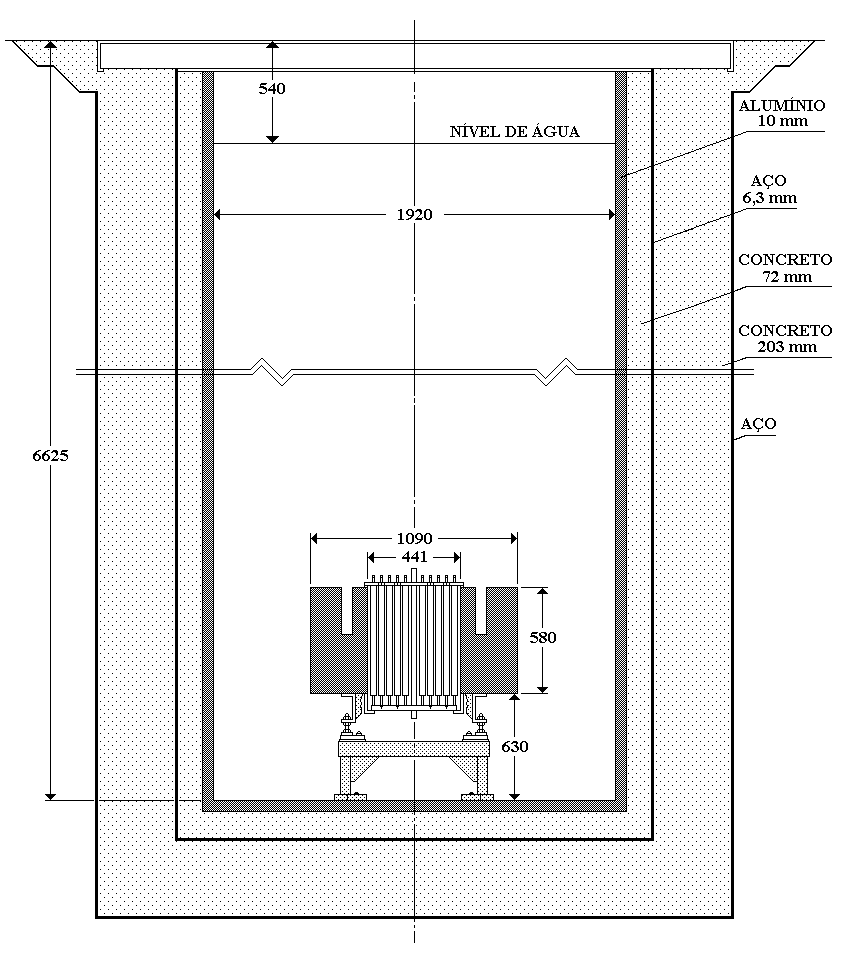
\includegraphics[scale=0.35]{figuras/poco_triga.png}
  \label{fig:poco_triga}
  \legend{Fonte: \cite{Veloso2005}}
\end{figure}

\begin{figure}[htb]
  \caption{Divisão do núcleo do reator TRIGA para cálculos de sub-canais \cite{Veloso2005}.}
  \centering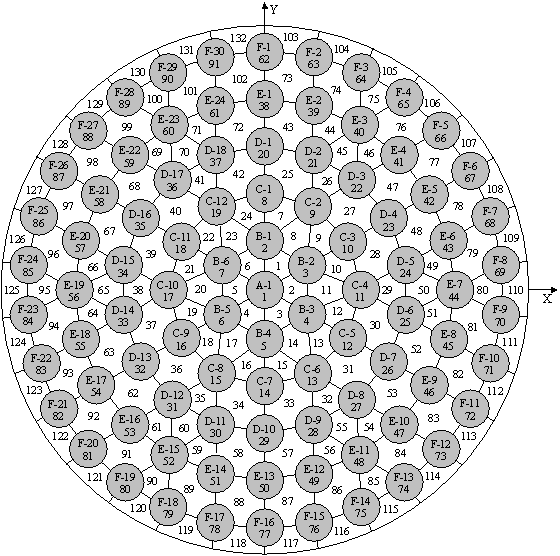
\includegraphics[scale=0.6]{figuras/subcanais_veloso.png}
  \label{fig:subcanais_veloso}
  \legend{Fonte: \cite{Veloso2005}}
\end{figure}

A temperatura média nos sub-canais foi calculada por Veloso \cite[Capítulo~8]{Veloso2005} com vistas ao licenciamento
do reator TRIGA IPR-R1 para operação a maior potência junto ao órgão fiscalizador. Sua metodologia
classificou cada um destes sub-canais, realizando cálculos levando
em consideração as propriedades físicas de cada um destes separadamente. Uma detalhada
explicação sobre métodos de cálculos por sub-canais com aplicação no reator TRIGA IPR-R1
pode ser encontrada na tese de Veloso \cite{Veloso2004}. Os resultados obtidos neste
trabalho, bem como as propriedades dos sub-canais e do núcleo do reator completo, são utilizados
como referência no desenvolvimento do modelo simplificado criado para a realização dos testes na
presente tese. A divisão original em sub-canais pode ser vista na Figura \ref{fig:subcanais_veloso}. Cabe
ressaltar que na modelagem simplificada foram utilizadas as características do escoamento do
sub-canal número $6$, mas a geometria foi modelada como um único pino cercado por água.

\section{Modelo}
%
% IMPORTANTE
%
% Separo th de neutronica em seções para colocar as seções de choque antes da neutrônica?
% Ou coloco logo as seções de choque antes de tudo?

Nesta seção é descrito o modelo físico e numérico utilizado nos testes do sistema acoplado.
O desenvolvimento deste modelo se deu de modo a balancear as características termo-hidráulicas
e neutrônicas desejáveis para um sistema de prova de conceito de cálculos acoplados
e as limitações técnicas impostas, tanto em relação à capacidade computacional disponível quanto
às limitações intrínsecas dos sistemas de \textit{software} utilizados.

\subsection{Fatores limitantes}
\label{ssec:lim}

O modelo de avaliação do acoplamento foi concebido de acordo com as restrições impostas pelos sistemas
utilizados na implementação do acoplamento. O \textit{OpenFOAM}, por se tratar de um sistema mais maduro
e com ampla rede de usuários, não impôs
restrições ao problema em termos de tamanho de malha a ser utilizada. Entretanto, a versão
do \textit{OpenFOAM} utilizada,
apresenta um erro (\textit{bug}, no jargão da Ciência da Computação) na implementação da resistência
de contato, o que inviabilizou a simulação do \textit{gap} existente no combustível. Essa foi a
primeira simplificação necessária no modelo em relação ao combustível do reator TRIGA IPR-R1.

No tocante ao \textit{milonga}, as restrições foram maiores. Foram duas as grandes limitações impostas
pelo \textit{milonga} na definição de um modelo mais complexo e computacionalmente exigente. A primeira
é relativa a execução de forma sequencial. Como o \textit{milonga} não é ainda capaz de executar de
forma paralela, o tamanho da malha a ser utilizada fica restrito à memória disponível.
O tamanho da malha também implica diretamente no tempo de execução.
Além disso, o \textit{milonga} ainda não é capaz de lidar com elementos prismáticos de forma confiável, limitando a
geração da malha por extrusão à utilização de elementos hexahédricos.
Como no caso de um combustível do tipo TRIGA o revestimento tem espessura ordens de grandeza
menor do que o raio do combustível, a não-utilização de elementos prismáticos impactou na geração
de uma malha mais refinada.

A segunda restrição imposta pelo \textit{milonga}, também em razão de um \textit{bug}, está na função
de acesso por coordenadas espaciais, fundamental para os cálculos acoplados com variação de seções de choque.
Este \textit{bug} limita o uso de regiões com o mesmo nome à regiões conectadas por elementos de malha.
Por exemplo, numa malha para todo o núcleo do reator TRIGA IPR-R1, são várias as regiões a serem definidas
como combustível, estando
tais regiões separadas por elementos de malhas de outras regiões. Neste caso, a função de acesso
à coordenadas espaciais do \textit{milonga} interrompe sua execução ao percorrer completamente a primeira
região encontrada com determinado nome, ignorando outras regiões com o mesmo nome.
Com isso, não é possível simular modelos de sub-canais
nem modelos do núcleo completo utilizando funções de coordenadas espaciais para cálculo de seções de choque.
Como o acoplamento, como previsto, necessita da atualização em todas as regiões definidas como combustível,
este \textit{bug} limitou o modelo a ser utilizado a um modelo com uma única região de
combustível\footnote{Durante a execução desta tese, alguns \textit{bugs} encontrados
  no \textit{milonga} foram corrigidos e
  reportados ao seu autor. Uma das correções acabou com um vazamento em memória que impedia que o \textit{milonga}
  fosse executado mais do que algumas vezes em modo iterativo.}.



%\footnote{É possível criar um modelo que trata cada combustível
%  individualmente, o que permitiria, por exemplo, diferenciar elementos de alumínio e aço-inoxidável tanto
%  para cálculos termo-hidráulicos quanto neutrônicos. Entretanto, dado o aumento no volume de definições
%  para os problemas termo-hidráulico e neutrônico,  o aumento na complexidade da implementação do acoplamento e
%  a necessidade de uma malha completado e refinada do núcleo, tal modelo foi considerado proibitivo.}


%Com estas limitações em mente, nas próximas seções será apresentado o modelo utilizado com todas as suas
%características bem como os parâmetros utilizados nas simulações neutrônica e termo-hidráulica.



\subsection{Modelo físico e numérico}
\label{ssec:mod_fis_num}

O modelo escolhido, de acordo com as limitações impostas já descritas,
representa um elemento combustível (elemento B6) do reator TRIGA IPR-R1, brevemente
apresentado na seção \ref{sec:triga}. Os combustíveis dos reatores do tipo TRIGA
possuem uma grande sensibilidade na sua
reatividade com a temperatura devido à já citada presença do hidreto de zircônio
em sua constituição. Essa característica intrínseca permite que pequenas
variações nas suas temperaturas levem a variações perceptíveis na neutrônica,
o que torna este modelo interessante para avaliação do acoplamento.

% Colocar figura do modelo completo

\begin{figure}[htb]
  \caption{Modelo: regiões e materiais. Em vermelho, combustível. Em amarelo, revestimento.
  em ciano, o refrigerante/moderador (água)}
  \centering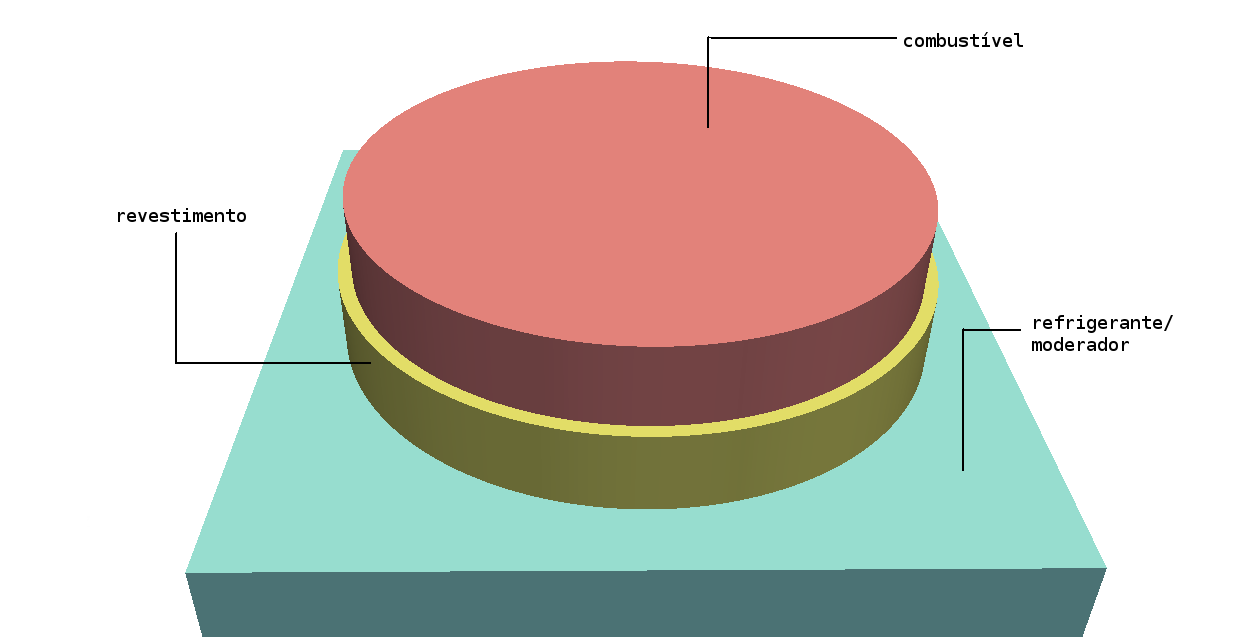
\includegraphics[scale=0.5]{figuras/regioes_surface2.png}
  \label{fig:regions}
%  \legend{Fonte: autor}
\end{figure}

\begin{figure}[htb]
  \caption{Vista isométrica do modelo completo.}
  \centering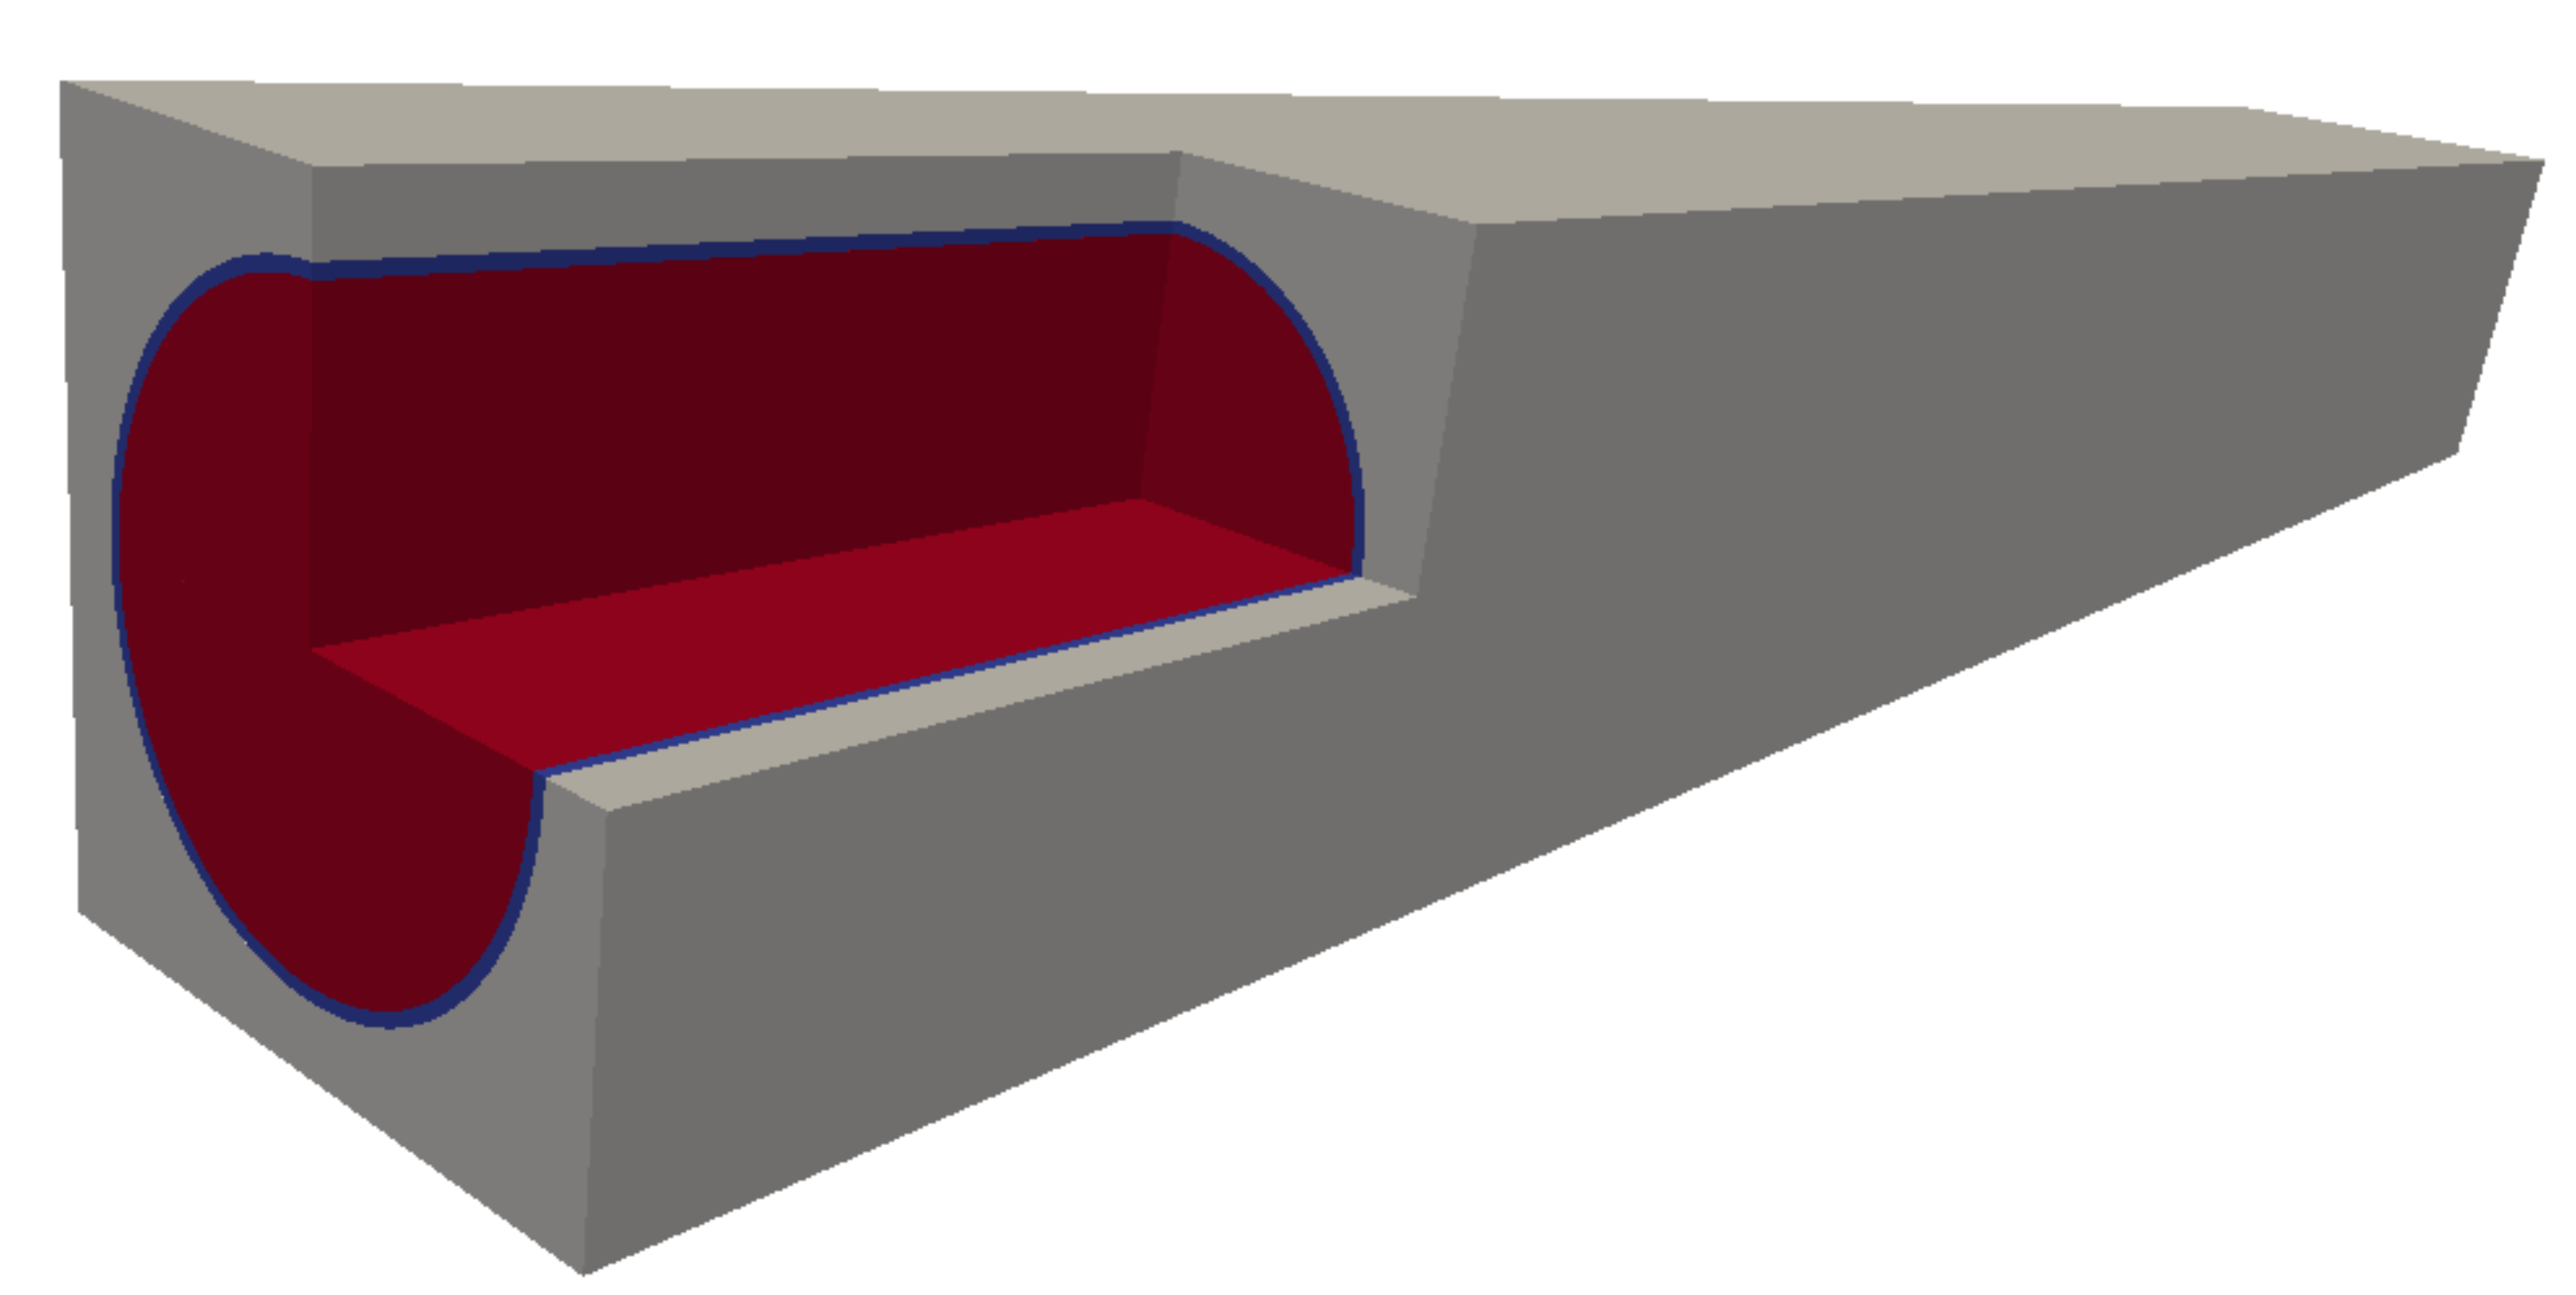
\includegraphics[scale=0.6]{figuras/all_regions_isometric.png}
  \label{fig:region_isometric}
%  \legend{Fonte: autor}
\end{figure}

\begin{figure}[htb]
  \caption{Discretização do modelo: regiões e materiais.}
  \centering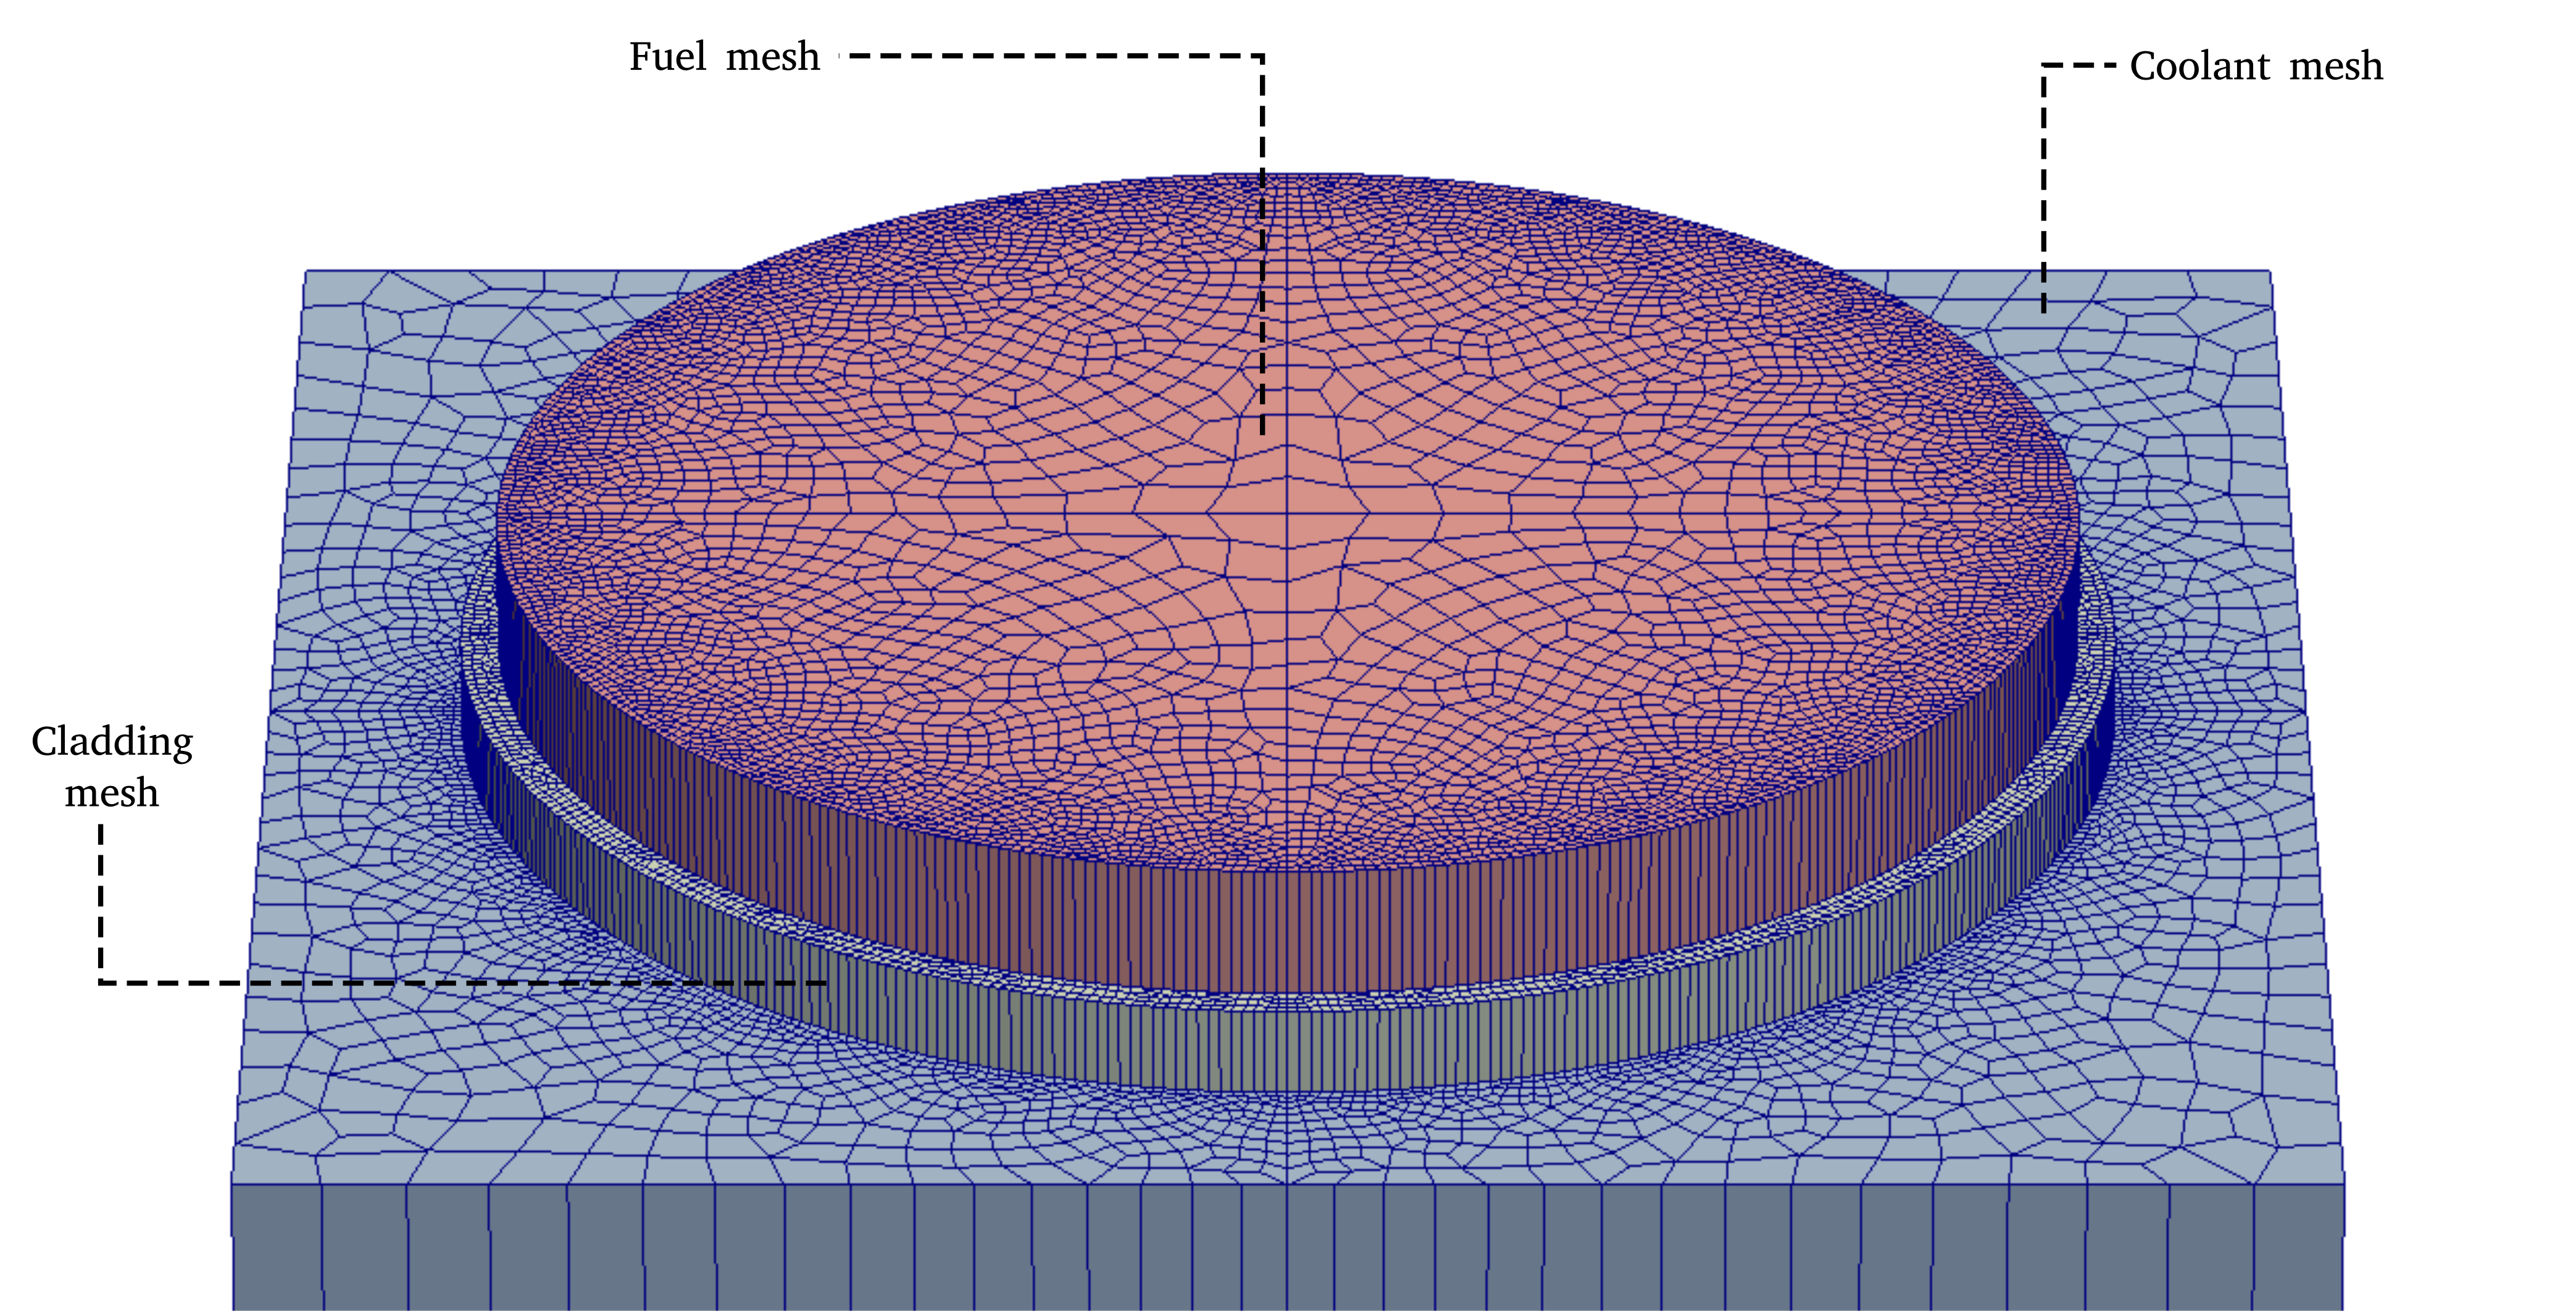
\includegraphics[scale=0.5]{figuras/regioes_edges_com_legenda_ingles.png}
  \label{fig:modelo_exploded}
%  \legend{Fonte: autor}
\end{figure}

O modelo consiste num combustível com revestimento de alumínio sem
o \textit{gap}, de modo que o diâmetro do combustível é mantido como no
combustível de referência e o diâmetro do \textit{gap} é estendido para
ocupar este espaço. Além disso, o modelo considera apenas o comprimento
ativo do combustível, sendo como um combustível mais curto. O volume
de água ao redor do combustível foi modelado considerando a razão entre
material físsil e moderador do núcleo completo do reator. Nenhuma outra
estrutura sólida, como discos de samário ou elementos estruturais, é
respresentada no modelo, sendo este idêntico axialmente em qualquer
altura, como observável nas Figuras \ref{fig:regions} e  e \ref{fig:region_isometric}.

\begin{table}[htb]
  \centering
  \caption[Medidas do modelo.]{Medidas do modelo.}
  \label{tab:size_model}
  \begin{tabular}{lr}
    Estrutura                         & {[}cm{]} \\ \hline
    Raio do combustível               & 1,78     \\
    Raio externo do revestimento      & 1,865    \\
    Arestas da região do refrigerante & 4,57     \\ \hline
    Altura do modelo do combustível   & 35,0    
  \end{tabular}
\end{table}

A malha gerada para o modelo foi construída por extrusão. Isso significa que
os elementos de malha foram gerados para uma superfície e a dimensão espacial
foi dada por um valor de comprimento e um número de camadas a serem geradas.
Foram geradas 35 camadas (cada uma com um $cm$), sendo o tamanho relativo
mínimo para elemento de malha de 0,5 e máximo de 4.0. Esses valores constrolam
o quanto o elemento próximo ao ponto com tal tamanho relativo crescerá durante
a geração da malha. A razão de crescimento entre o refinamento do revestimento
e as áreas restantes foi estabelecido em 1,2. Com isso, foi possível conseguir
elementos suficientemente pequenos para realizar os cálculos na região
do revestimento e ainda obter uma malha com tamanho tratável pelo \textit{milonga}.
A malha gerada tem 346.675 elementos.

As dimensões da malha do modelo geram implicações nos resultados dos cálculos, em
especial a pequena granularidade axial (35 camadas). Esta granularidade
pode ser observada na Figura \ref{fig:modelo_exploded},
na qual é possível notar
o refinamento entre as diversas regiões e, em contraste, o tamanho dos elementos logitudinalmente.
Entretanto, mesmo com tais
limitações impostas pelo \textit{milonga} na sua capacidade de lidar
com malhas de muitos elementos, é possível utilizar a malha gerada para verificar
as diferenças nos resultados dos cálculos entre um sistema não acoplado e outro acoplado.


\subsection{Condições de contorno e parâmetros numéricos: termo-hidráulica}
\label{subsec:ccth}


São quatro condições de contorno utilizadas na solução da simulação termo-hidráulica
nas superfícies que limitam o domínio. As extremidades do combustível e do revestimento
são definidas como adiabáticas. Nas
extremidades da região do refrigerante (água), são definidos entrada (\textit{inlet}) e
saída (\textit{outlet}) para o escoamento. As laterais do modelo são definidas
como simétricas. Na figura \ref{fig:ccth} são mostradas as condições de contorno
utilizadas e as regiões correspondentes. As superfícies definidas como simétricas (\textit{symmetry})
estão em vermelho
enquanto em azul estão a entrada e saída de fluido. A região sólida representa o
combustível e revestimento, ambos com condiçoes de contorno adiabáticas nas extremidades.

\begin{figure}[htb]
  \caption{Modelo: condições de contorno da simulação termo-hidráulica e regiões
    correspondentes.}
  \centering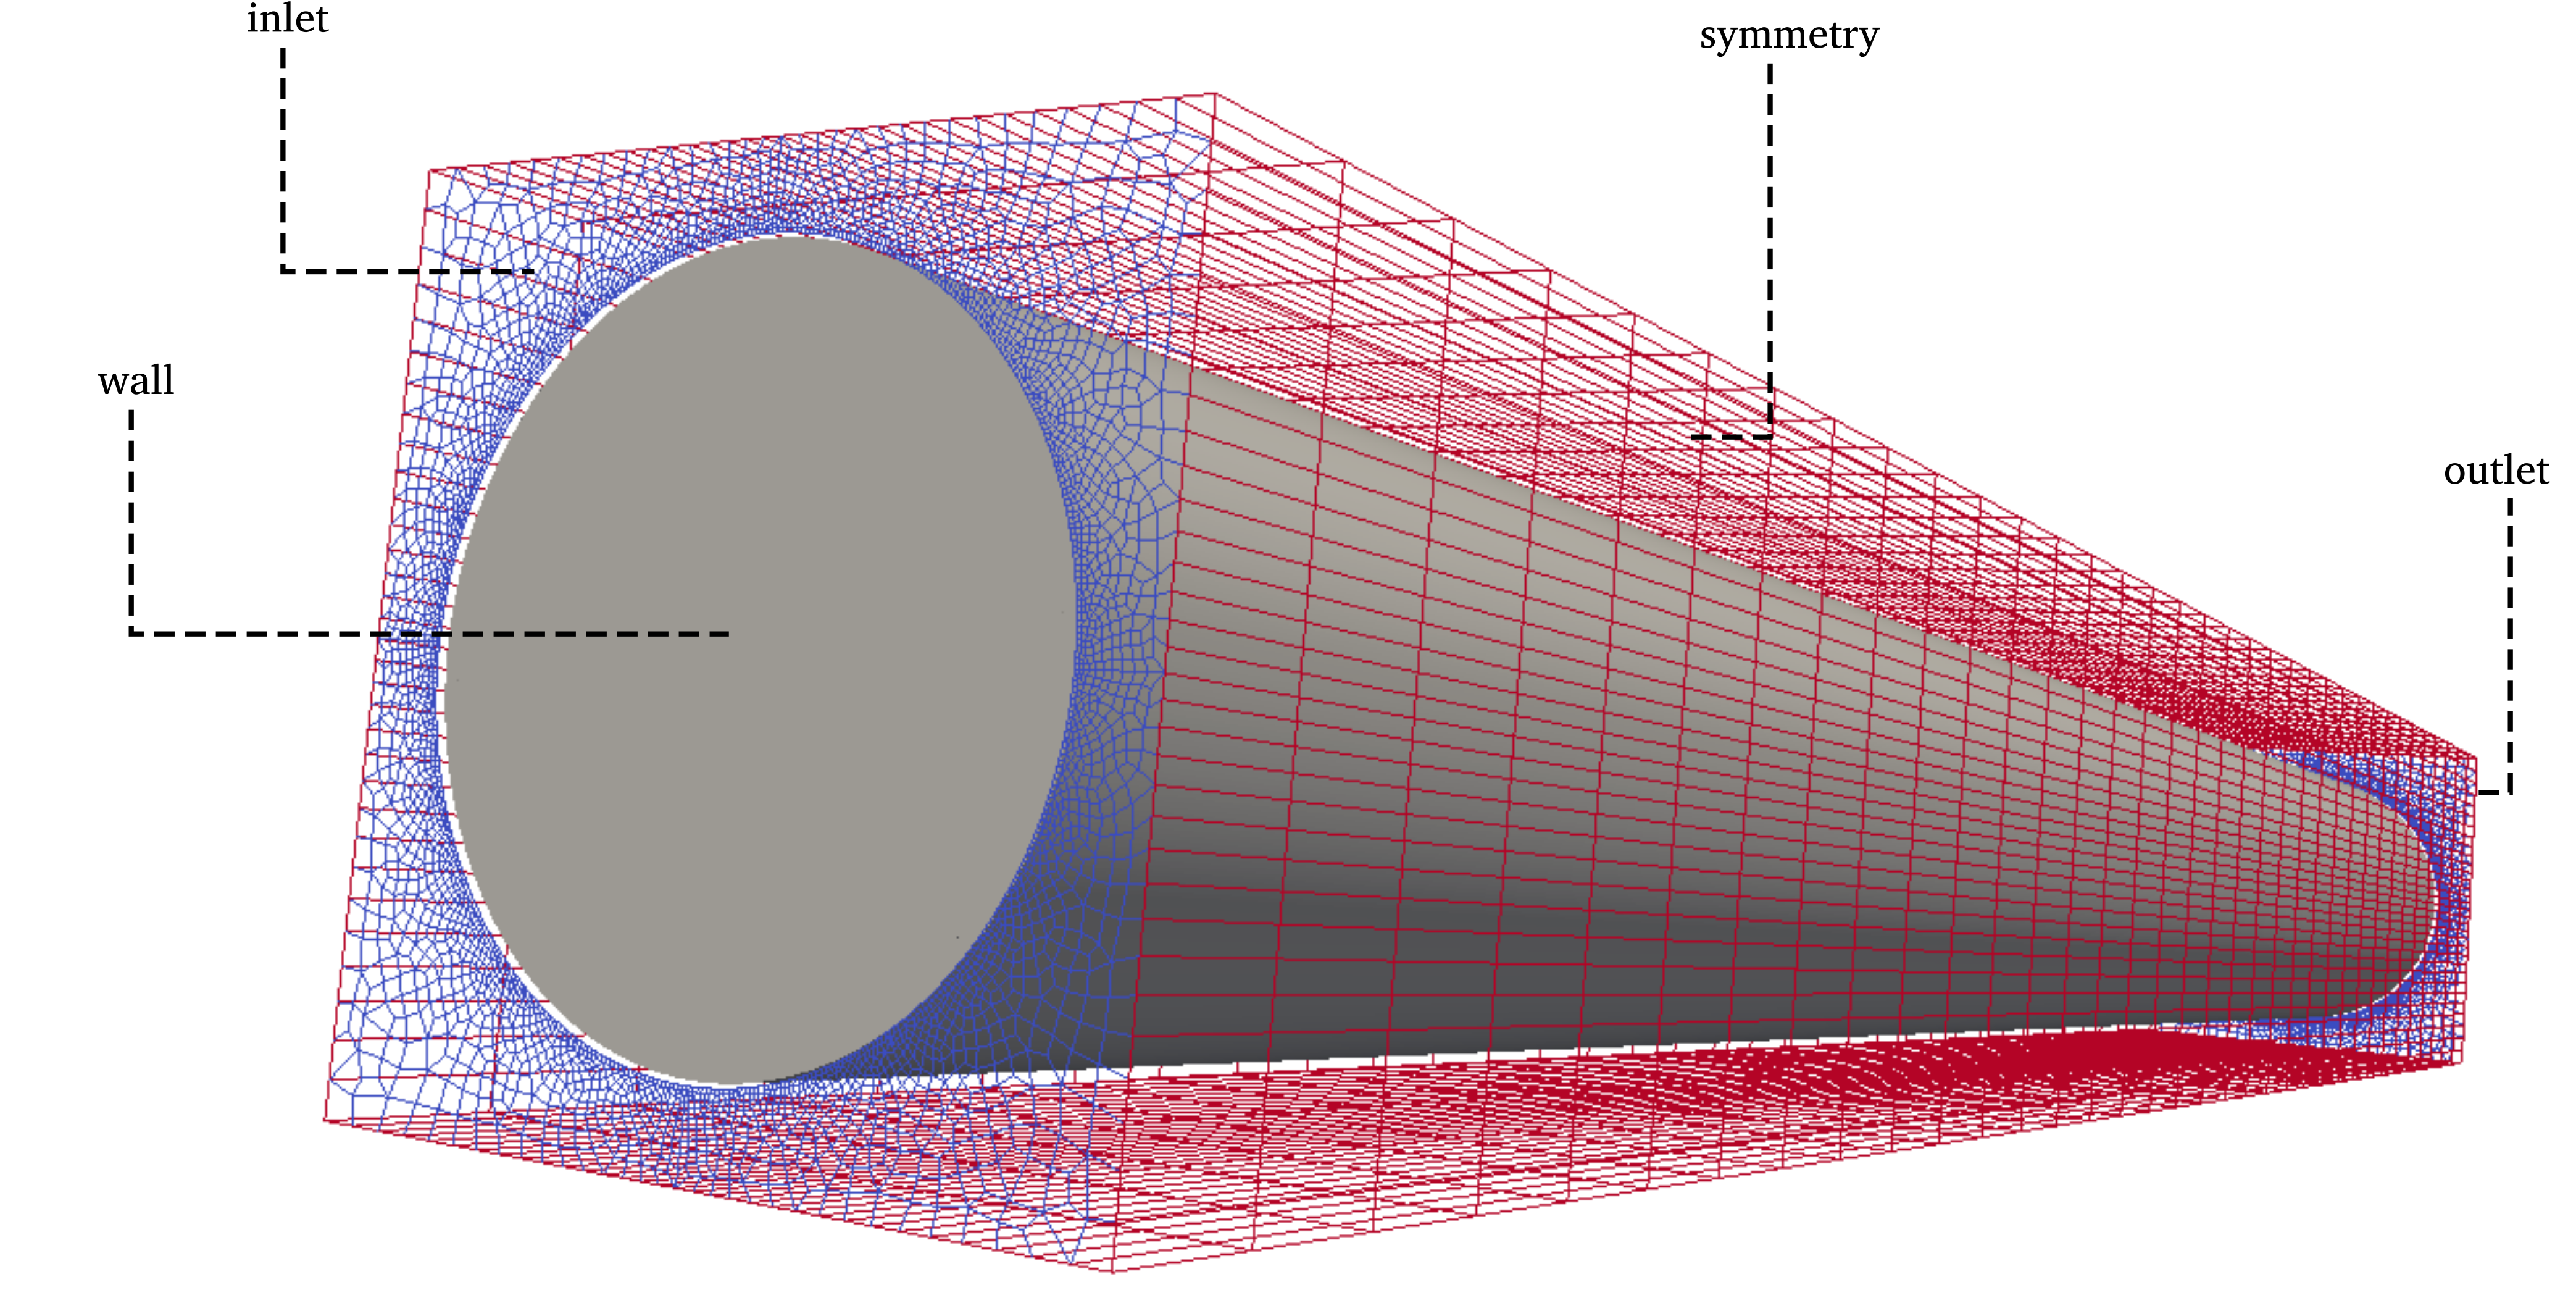
\includegraphics[scale=0.5]{figuras/inlet_paredes_extremos_wireframe2.png}
  \label{fig:ccth}
%  \legend{Fonte: autor}
\end{figure}

As superfícies entre regiões têm suas condições de contorno definidas automaticamente
num dos passos da etapa de pré-processamento. Por definição, o \textit{OpenFOAM} importa
a malha num único conjunto de elementos, armazenando as definições de regiões
contidas na malha. Um dos utilitários disponibilizados pelo \textit{OpenFOAM} separa
as regiões, gerando condições de contorno em cada uma das regiões que representam
as interfaces entre regiões. Outro utilitário é utilizado em seguida para definir valores
para os parâmetros das respectivas condições de contorno, de acordo com as definições
previamente feitas pelo usuário. Como resultado do pré-processamento
entre regiões, são obtidas condições de contorno que implementam a troca
conjugada de calor entre as distintas regiões. Na tabela \ref{tab:cc-superf} são
apresentadas as condições de contorno utilizadas nas superfícies entre regiões para a temperatura.
É possível perceber que todas as superfícies,
tanto para campos sólidos e fluidos, utilizam a mesma condição de contorno:
\texttt{compressible::turbulentCoupledBaffleMixed}.
%\begin{itemize}
%\item \texttt{compressible::turbulentCoupledBaffleMixed}.
%\end{itemize}

\begin{table}[htb]
\centering
\caption{Condições de contorno entre superfícies internas (pré-processamento)}
\label{tab:cc-superf}
\begin{tabular}{llcc}
\multicolumn{1}{c}{Região}    & \multicolumn{1}{c}{Superfície} & \begin{tabular}[c]{@{}c@{}}Condição\\ de contorno\end{tabular}                                        & Campo              \\ \hline
Combustível                   & \textit{fuel\_to\_cladding}    & \multirow{4}{*}{\begin{tabular}[c]{@{}c@{}}compressible::\\ turbulentCoupledBaffleMixed\end{tabular}} & \multirow{4}{*}{T} \\ \cline{1-2}
\multirow{2}{*}{Revestimento} & \textit{cladding\_to\_fuel}    &                                                                                                       &                    \\
                              & \textit{cladding\_to\_coolant} &                                                                                                       &                    \\ \cline{1-2}
Refrigerante                  & \textit{coolant\_to\_cladding} &                                                                                                       &                   
\end{tabular}
\end{table}
As condições de contorno devem ser estabelecidas para todas as grandezas sendo calculadas. Algumas
destas grandezas, como a potência ($Q$), por exemplo, são automaticamente calculadas nas superfícies a partir
dos campos internos. Entretanto, isto não desobriga o usuário de explicitamente definí-las como \textit{calculated}.

Esta condição de contorno utiliza as
propriedades termofísicas dos respectivos materiais, que são previamente definidas na
modelagem do problema, para o cálculo do fluxo de calor entre as regiões. As propriedades termofísicas
dos materiais utilizados por este modelo são dadas na tabela \ref{tab:termofisica}.



\begin{table}[htb]
\centering
\caption{Propriedades termofísicas dos materiais em função da temperatura ($T$)}
\label{tab:termofisica}
\begin{tabular}{lllll}
Material     & \begin{tabular}[c]{@{}l@{}}Densidade\\ {[}$kg/m^3${]}\end{tabular} & \begin{tabular}[c]{@{}l@{}}Calor específico\\ {[}$kJ/kg.K${]}\end{tabular} & \begin{tabular}[c]{@{}l@{}}Condutividade\\ {[}$W/m.K${]}\end{tabular}      & \begin{tabular}[c]{@{}l@{}}Viscosidade\\ {[}$\mu Pa.s${]}\end{tabular} \\
\hline
Combustível  & 6280                                                               & \begin{tabular}[c]{@{}l@{}}$0,294$+\\ 6.,196 x $10^{-4} T-$\\2,748 x $10^{-9} T^2+$\\1,354 x $10^{-11} T^3$\end{tabular}              & \begin{tabular}[c]{@{}l@{}}22,872-\\ 4,3131 x $10^{-2} T +$ \\1,124 x $10^{-4} T^2-$\\1,0039 x $10^{-11} T^3$\end{tabular}              & -                                                                     \\
\hline
Revestimento & 2705                                                               & \begin{tabular}[c]{@{}l@{}}$0,892$+\\4,44361 x $10^{-4} T+$\\3,632 x $10^{-8} T^2$\end{tabular}                & \begin{tabular}[c]{@{}l@{}}223,7+\\ 4.756 x $10^{-2}T+$\\ 1,0215 x $10^{-5} T^2-$\\ 1,8887 x $10^{-11} T^3$
  \end{tabular} & -                                                                     \\
\hline
        Refrigerante & 995                                                                & 4,18                                                                       & 0,62                                                                       & 797                                                                  
\end{tabular}
\end{table}



As principais condições de contorno e iniciais do problema apresentado estão definidas na tabela \ref{tab:cc-init}.
Estas condições descrevem as características iniciais do problema sendo resolvido. Alguns comentários sobre sobre
a tabela \ref{tab:cc-init}: o velocidade na entrada do sistema se baseia na velocidade média do escoamento na
entrada do núcleo do reator \cite{Veloso2005}. A região do revestimento, por ser sólida, herda a implementação
do termo-fonte. Entretanto, este é mantido nulo já que não há geração de energia no revestimento. A campo
interno inicial de potência é \textbf{não-uniforme} e definido como variável. A campo não-uniforme permite estabelecer
uma condição inicial de campo heterogêneo, tal como uma distribuição volumétrica de potência. O valor para este
campo é definido como \textbf{variável}, já que esta distribuição de potências varia para cada diferente simulação.

Vale ressaltar que a potência, tal qual implementada no \textit{solver}, é dada em $W$ por $m^3$.

\begin{table}[htb]
\centering
\caption{Condições de contorno iniciais para a termo-hidráulica}
\label{tab:cc-init}
\begin{tabular}{llllc}
Region                    & Field                   & Boundary      & Type         & Value                 \\
\hline
\multirow{6}{*}{coolant}  & \multirow{2}{*}{T}      & inlet         & fixedValue   & $300K$                  \\
                          &                         & outlet        & zeroGradient & -                     \\
                          & \multirow{2}{*}{U}      & inlet         & fixedValue   & 0.1 {[}$m/s${]}         \\
                          &                         & outlet        & zeroGradient & -                     \\
                          & \multirow{2}{*}{p\_rgh} & inlet         & zeroGradient & -                     \\
                          &                         & outlet        & fixedValue   & 0 {[}$kg/m.s^2 = Pa${]}  \\
\hline
\multirow{3}{*}{cladding} & T                       & wall          & zeroGradient & -                     \\
                          & \multirow{2}{*}{Q}      & wall          & calculated   & -                     \\
                          &                         & internalField & uniform      & 0 {[}$W/m^3${]}          \\
\hline
\multirow{3}{*}{fuel}     & T                       & wall          & zeroGradient & -                     \\
                          & \multirow{2}{*}{Q}      & wall          & calculated   & -                     \\
                          &                         & internalField & non-uniform  & (variable) {[}$W/m^3${]}
\end{tabular}
\end{table}

O escoamento do fluido no modelo é considerado turbulento, baseado nas condições usuais de operação
do reator TRIGA IPR-R1 \cite{Veloso2005}. A turbulência foi modelada utilizando-se o modelo
$\kappa-\epsilon$ \cite{Launder1974}, que assume que a viscosidade turbulenta está relacionada
à energia cinética ($\kappa$) e dissipação ($\epsilon$).

Uma vez definidas as características físicas do modelo e as condições iniciais e de contorno,
o problema está fechado e é possível iniciar os cálculos propriamente ditos.

Entretanto, para isso, são necessárias, além das configurações relativas
ao problema físico, as definições relativas aos esquemas de discretização a serem utilizados e aos
algoritmos numéricos a serem utilizados. Entenda-se por esquemas de discretização, 

Complementando a breve introdução ao método de volumes finitos
dada no capítulo \ref{chap:teoria} desta tese, são apresentados na tabela \ref{tab:discretizacao}
os esquemas de discretização utilizados nos cálculos acoplados e não acoplados. O manual
do programadar do \textit{OpenFOAM} \cite[Seção 2.4]{OpenFOAM2015b} descreve com detalhes alguns
dos métodos de discretização de equações disponíveis na ferramenta.


\begin{table}[htb]
\centering
\caption{Esquemas de discretização utilizados nos cálculos de volumes finitos}
\label{tab:discretizacao}
\begin{tabular}{cccccc}
\multicolumn{1}{l}{} & \multicolumn{5}{c}{\textbf{Termo da equação}}                                                                                                                                                                                                                                                   \\ \cline{2-6} 
\textbf{Região}      & $\nabla \phi$                                                   & $\nabla . \phi$                                                              & $\nabla^2 . \phi$                                                           & interpolação & \begin{tabular}[c]{@{}c@{}}normal à\\ face da célula\end{tabular} \\ \hline
Combustível          & Gauss linear                                                & -                                                                       & \begin{tabular}[c]{@{}c@{}}Gauss linear\\ não-corrigido\end{tabular} & linear       & não-corrigido                                                     \\ \hline
Revestimento         & Gauss linear                                                &                                                                         & \begin{tabular}[c]{@{}c@{}}Gauss linear\\ não-corrigido\end{tabular} & linear       & não-corrigido                                                     \\ \hline
Refrigerante         & \begin{tabular}[c]{@{}c@{}}Mínimos\\ quadrados\end{tabular} & \textit{\begin{tabular}[c]{@{}c@{}}Bounded\\ Gauss upwind\end{tabular}} & \begin{tabular}[c]{@{}c@{}}Gauss linear \\ limitado 1.0\end{tabular} & linear       & limitada 1.0                                                     
\end{tabular}
\end{table}

Os esquemas utilizados na solução do problema apresentado foram escolhidos na tentativa de manter
um compromisso entre o tempo de execução e qualidade da solução (em termos de erros inerentes
aos métodos de discretização). Por se tratar de um problema conceitual, como extensamente mencionado,
a ideia por detrás da escolha dos métodos de discretização foi de interferir o mínimo possível com
os valores padrão do \textit{solver} utilizado e, ao mesmo tempo, garantir que o termo-fonte
adicionado não impactasse negativamente o processo de obtenção da solução numérica.


% --------------------------------- NEUTRONICA -----------------------------------------%
\subsection{Condições de contorno e parâmetros numéricos: neutrônica}
\label{ssec:neutro}

O \textit{milonga} convenientemente trata internamento as condições de contorno
entre as diferentes regiões, ou materiais, do ponto de vista dos cálculos neutrônicos,
poupando o usuário de certa quantidade de trabalho extra e evitando introdução
de erros de modelagem. Desse modo, é suficiente definir as condições de contorno
para as superfícies externas do domínio.

\begin{table}[htb]
  \centering
\caption{Condições de contorno da neutrônica}
\label{tab:cc-neut}
\begin{tabular}{ccc}
Fronteira         & Tipo                             & Região correspondente         \\ \hline
\textit{inlet}    & \multirow{2}{*}{\textit{Vacuum}} & \multirow{2}{*}{Refrigerante} \\
\textit{outlet}   &                                  &                               \\ \cline{1-1}
\textit{extremes} & \textit{Vacuum}                  & Revestimento e combustível    \\ \hline
\textit{walls}    & \textit{Mirror}                  & Refrigerante                 
\end{tabular}
\end{table}

As condições de contorno que podem ser usadas são de um fluxo imposto (Dirichlet),
uma corrente imposta (Neumann) ou uma combinação linear destas (Robin). A condição de
fluxo se limita a fluxo zero na fronteira. Esta condição é aplicada utilizando-se
a palavra-chave \textit{vacuum} dentro do \textit{milonga}, enquanto a condição
de corrente deve ter derivada zero na direção da normal à fronteira e é utilizada
pela palavra-chave \textit{mirror}. Caso se deseje utilizar a condição mixta, deve
ser utilizada a palavra-chave \textit{robin} seguida do um argumento de ponto
flutuante entre zero e um.

As condições de contorno utilizadas no modelo utilizado estão listadas na Tabela
\ref{tab:cc-neut}. Na figura \ref{fig:cc-neut} podem ser vistas na metade à esquerda
a malha e as condições de contorno utilizadas enquanto na metade direita as
regiões correspondentes a cada material.

\begin{figure}[htb]
  \caption{Vista superior do modelo de combustível apresentando as distintas regiões e condições de contorno
    sobre a malha bidimensional.}
  \centering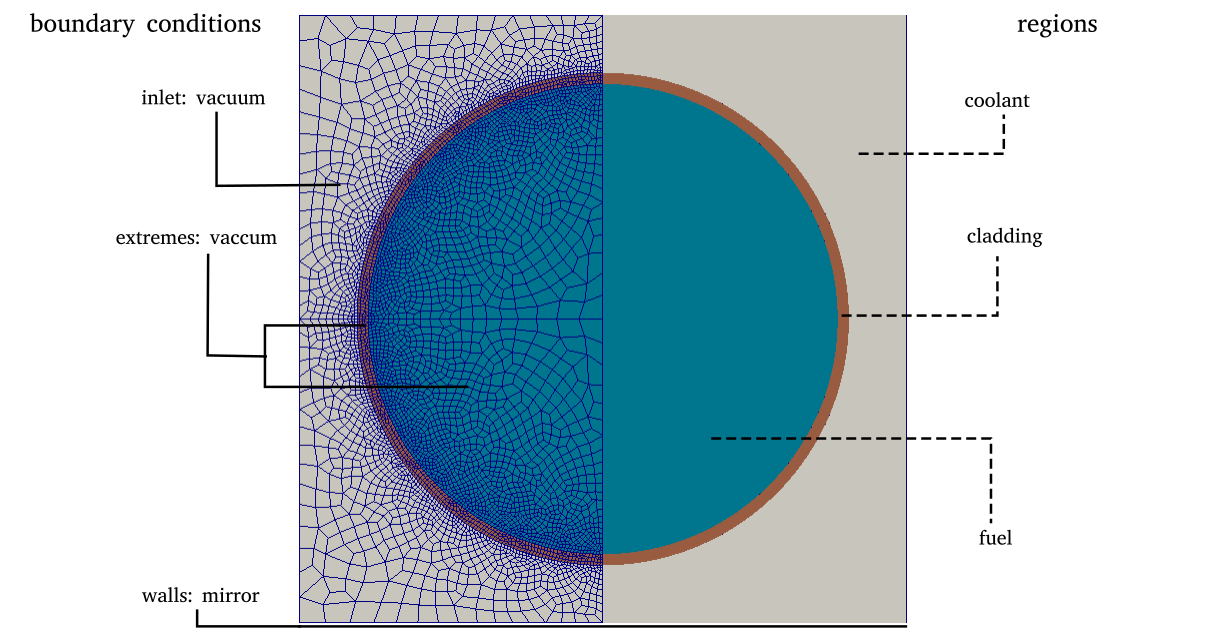
\includegraphics[scale=0.52]{figuras/regions_neutronica_malha_e_sem.png}
  \label{fig:cc-neut}
%  \legend{Fonte: \cite{Veloso2005}}
\end{figure}

% Colocar um exemplo aqui?
% Ou uma figura?

% --------------------------------- SECOES DE CHOQUE -----------------------------------------%
\section{Geração de seções de choque}
\label{sec:gerxs}

A fim de verificar o impacto das variações de temperatura obtidas nos cálculos
termo-hidráulicos no fluxo
neutrônico e, portanto, na potência volumétrica, é necessário utilizar seções de choque
fisicamente compatíveis com o problema a ser resolvido. A breve introdução dada sobre
neutrônica na seção \ref{sec:neutronica} desta tese descreve a importância das seções
de choque no cálculo neutrônico. As seções de choque surgem no cálculo neutrônico
pela aproximação por difusão como coeficientes dos distintos termos da equação
diferencial que resolve o fluxo de nêutrons.

O \textit{milonga} utiliza mnemônicos específicos para cada coeficiente, de modo
que estes possam ser representados, tanto como valores constantes, como por funções
de temperatura, por exemplo, assim utilizados na modelagem nesta tese. Na tabela
\ref{tab:coeff-dif} estão apresentados os mnemônicos utilizados pelo \textit{milonga}
no modelo utilizado bem como a divisão de grupos em energias.

% Tabela para os valores
\begin{table}[htb]
  \centering
  \caption[Coeficientes da Equação de Difusão.]{Coeficientes da Equação de Difusão.}
  \label{tab:coeff-dif}
  \begin{tabular}{ l | c | r}
  \hline
  \multicolumn{3}{ c }{Coeficientes Mnemônicos} \\
  \hline
  \multirow{4}{*}{Grupo 1: > 0,625 MeV} & Coeficiente de Difusão & $D1$\\
& Seção de choque de absorção & $\Sigma A1$\\
& Seção de choque de espalhamento & $\Sigma S1.2$\\
  & Neutrons por fissão * Seção de choque de fissão & $\nu \Sigma F1$\\
  \hline
\multirow{3}{*}{Grupo 2: < 0,625 MeV} & Coeficiente de difusão & $D2$\\
& Seção de choque de absorção & $\Sigma A2$\\
& Neutrons por fissão * Seção de choque de fissão & $\nu \Sigma F2$ \\
\hline
\end{tabular}
\end{table}

Para a geração das seções de choque, um modelo bidimensional com propriedades
equivalentes ao modelo tridimensional a ser simulado
foi definido. Esta equivalência foi garantida mantendo-se a proporção entre material
físsil e moderador em ambos os modelos. Com base nessa proporção,
todos os materiais foram definidos como anéis concêntricos. 

Uma vez definida a geometria,
foram definidas quatro diferentes temperaturas cobrindo a faixa de operação
do reator TRIGA IPR-R1. A menor temperatura sendo a temperatura ambiente até
a temperatura próxima a máxima do combustível do TRIGA IPR-R1 em operação
a $250 kW$ \cite{Veloso2005}, num grupo de quatro, apresentado na tabela
\ref{tab:temp}.

\begin{table}[htb]
\centering
\caption{Temperaturas de referência para os materiais.}
\label{tab:temp}
\begin{tabular}{lrrrr}
\multicolumn{5}{c}{Temperaturas dos materiais}                                                                                                       \\ \hline
             & \multicolumn{1}{l}{$T_1${[}K{]}} & \multicolumn{1}{l}{$T_2${[}K{]}} & \multicolumn{1}{l}{$T_3${[}K{]}} & \multicolumn{1}{l}{$T_4${[}K{]}}      \\ \hline
Combustível  & 300                             & 400                             & 500                             & 600                             \\ \hline
Revestimento & 300                             & 396                             & 403                             & 410                             \\ \hline
Refrigerante & 300                             & 308,5                           & 317                             & 341                            
\end{tabular}
\end{table}

A metodologia utilizada para a geração de seções de choque \cite{Reis2015}
foi desenvolvida pelo grupo de física de reatores do DEN/UFMG. Esta metodologia
utiliza o código WIMSD-5B \cite{Halsall1986} para gerar seções de choque dependentes da temperatura
para materias específicos e para variado número de grupos de energia. No presente
trabalho, foram utilizados dois grupos de energia separados em 0,625 Mev como
apresentado na tabela \ref{tab:coeff-dif}. A composição dos materiais utilizados,
em especial o combustível, que contem mais isótopos, se baseou na composição
isotópica do reator TRIGA IPR-R1 no ano de 2004. Estas composições, massa e código
de material utilizados na geração de seções
de choque pelo WIMSD-5B estão na Tabela \ref{tab:composicao}.


\begin{table}[htb]
  \centering
  \caption{Composição dos materiais para geração de seções de choque com o WIMSD-5B \cite{Halsall1986, Reis2015}}
  \label{tab:composicao}
\begin{tabular}{rlcr}
                              & \multicolumn{1}{c}{Material}                                         & Código & \multicolumn{1}{c}{Massa} \\ \cline{2-4} 
\multirow{4}{*}{Combustível}  & \begin{tabular}[c]{@{}l@{}}H (no hidreto\\ de zircônio)\end{tabular} & 5001   & $3,7525e^{-02}$           \\
                              & Zr                                                                   & 91     & $3,7727e^{-02}$           \\
                              & U$^{235}$                                            & 2235   & $2,5744e^{-04}$           \\
                              & U$^{238}$                                            & 8238   & $1,0167e^{-03}$           \\ \hline
Revestimento                  & Al                                                                   & 27     & $6,0261e^{-02}$           \\ \hline
\multirow{2}{*}{Refrigerante} & H                                                                    & 3001   & $6,6653e^{-02}$           \\
                              & O                                                                    & 6016   & $3,3327e^{-02}$          
\end{tabular}
\end{table}


As temperaturas utilizadas na geração das seções de choque
e as seções de choque resultantes são apresentadas nas tabelas \ref{tab:temp-fuel},
\ref{tab:temp-cladding} e \ref{tab:temp-coolant} respectivamente para o combustível, revestimento
e moderador.


\begin{table}[htb]
  \centering
  \caption[Temperaturas para combustível.]{Temperaturas para o combustível}.
  \label{tab:temp-fuel}
  \begin{tabular}{r r r r r}
  \multicolumn{5}{c}{Combustível} \\
  \hline
  Parâmetro & $300K$ & $400K$ & $500K$ & $600K$ \\
  \hline
  $D1$ & 0,0108349 & 0,0108521 & 0,0108489 & 0,010846\\
  $\Sigma A1$ & 0,771135 & 0,783626 & 0,795686 & 0,806567\\
  $\Sigma S1.2$ & 3,3991 & 3,4329 & 3,4264 & 3,4206\\
  $\nu \Sigma F1$ & 0,500982 & 0,500304 & 0,500377 & 0,500441\\
  \hline
  $D2$ & 0,00314942 & 0,0031682 & 0, 0032163 & 0,0032743 \\
  $\Sigma A2$ & 11,0389 & 10,8142 & 10,4004 & 9,90199\\
  $\nu \Sigma F2$ & 20,1943 & 19,7703 & 18,9898 & 18,0499\\
  \hline
\end{tabular}
\end{table}

\begin{table}[htb]
  \centering
  \caption[Temperaturas para o revestimento.]{Temperaturas para o revestimento}.
  \label{tab:temp-cladding}
  \begin{tabular}{r r r r r}
    \multicolumn{5}{c}{Revestimento} \\
    \hline
    Parâmetro & $300K$ & $396K$ & $403K$ & $410K$ \\
    \hline
    $D1$ & 0,0299644 & 0,0299699 & 0,0299678 & 0,0299659 \\
    $\Sigma A1$ & 0,0288617 & 0,028926 & 0,0289199 & 0,0289143 \\
    $\Sigma S1.2$ & 3,3991 & 3,4329 & 3,4264 & 3,4206\\
    \hline
    $D2$ & 0,0376276 & 0,0376721 & 0,0377696 & 0,0379140\\
    $\Sigma A2$ & 0,874322 & 0,865956 & 0,846858 & 0,818690\\
    \hline
  \end{tabular}
\end{table}

\begin{table}[htb]
  \centering
  \caption[Temperaturas para o refrigerante.]{Temperaturas para o refrigerante}.
  \label{tab:temp-coolant}
  \begin{tabular}{r r r r r}
    \multicolumn{5}{c}{Moderador} \\
    \hline
    Parâmetro & $300K$ & $308,5K$ & $317K$ & $341K$ \\
    \hline
    $D1$ & 0,0126587 & 0,0126685 & 0,0126696 & 0,0126705\\
    $\Sigma A1$ & 0,0290925 & 0,0292130 & 0,0292018 & 0,0291917\\
    $\Sigma S1.2$ & 3,3991 & 3,4329 & 3,4264 & 3,4206\\
    \hline
    $D2$ & 0,00213616 & 0,0021262 & 0021368 & 0021589\\
    $\Sigma A2$ & 1,42651 & 1,41891 & 1,39505 & 1,35409\\
    \hline
  \end{tabular}
\end{table}


Devido a uma limitação do código WIMSD-5B na geração de seções de choque de espalhamento
para cada material separadamente, as seções de choque de
espalhamento foram geradas para uma homogeneização dos materiais em uma única célula,
sendo esta a razão dos valores serem os mesmos para todos os materiais.

%
% IMPORTANTE: Talvez este próximo parágrafo não deva ficar aqui, mas no modelo da neutrônica.
%
As seções de choque obtidas foram então escritas no formato \textit{milonga} como
funções de uma variável dependentes da temperatura. Como o milonga tem informação
das células em relação à malha, a temperatura de cada célula é argumento da
função de uma variável dependente da temperatura. Se a temperatura não está
exatamente tabulada, o \textit{milonga} provê interpolação linear por padrão.

É exatamente esta característica do \textit{milonga} que permite o cálculo neutrônico
independente por elemento de volume, sendo possível obter variações detalhadas
de acordo com a granularidade da malha utilizada pelo modelo.
